\documentclass[]{article}
\usepackage[utf8]{inputenc} % allow utf-8 input
\usepackage[T1]{fontenc}    % use 8-bit T1 fonts
\usepackage{hyperref}       % hyperlinks
\usepackage{url}            % simple URL typesetting
\usepackage{booktabs}       % professional-quality tables
\usepackage{amsfonts}       % blackboard math symbols
\usepackage{nicefrac}       % compact symbols for 1/2, etc.
\usepackage{microtype}      % microtypography
\usepackage{graphicx}
\usepackage{caption}
\usepackage{subcaption}
\usepackage{pgffor} % for loop
\usepackage{xstring} % for declaring lists



\graphicspath{{figures/}}


\title{Generalisation report}

\author{%
	report produced from \href{https://github.com/bethgelab/google_scholar_crawler}{google\_scholar\_crawler}\\
}



\begin{document}

\newcommand{\figwidth}{0.24\textwidth}
\newcommand{\captionspace}{-1.5\baselineskip}
\newcommand{\captionspaceII}{0.6\baselineskip}
\newcommand{\captionspaceBenchmark}{-0.5\baselineskip}


\maketitle
\begin{figure}
    \centering
    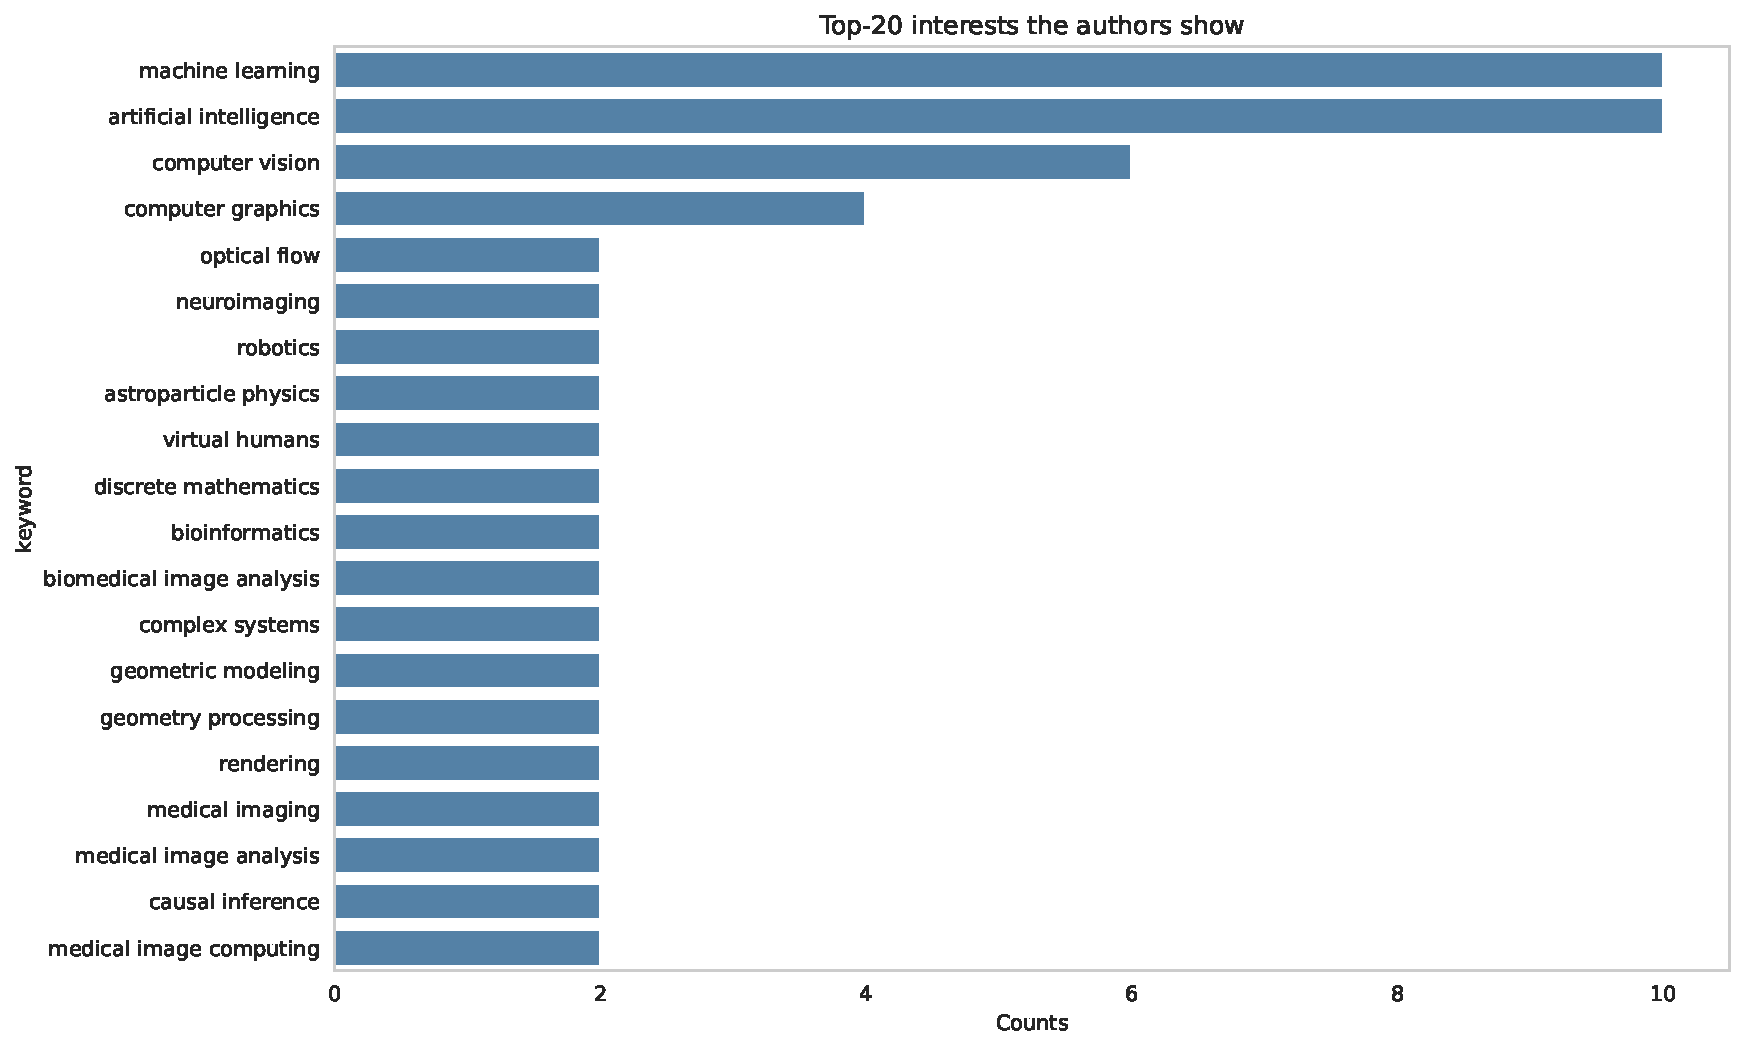
\includegraphics[width=0.8\linewidth]{figures/top-keywords.pdf}
    \caption{Top Keywords of the extracted authors}
    \label{fig:top-keywords}
\end{figure}
\begin{figure}
    \centering
    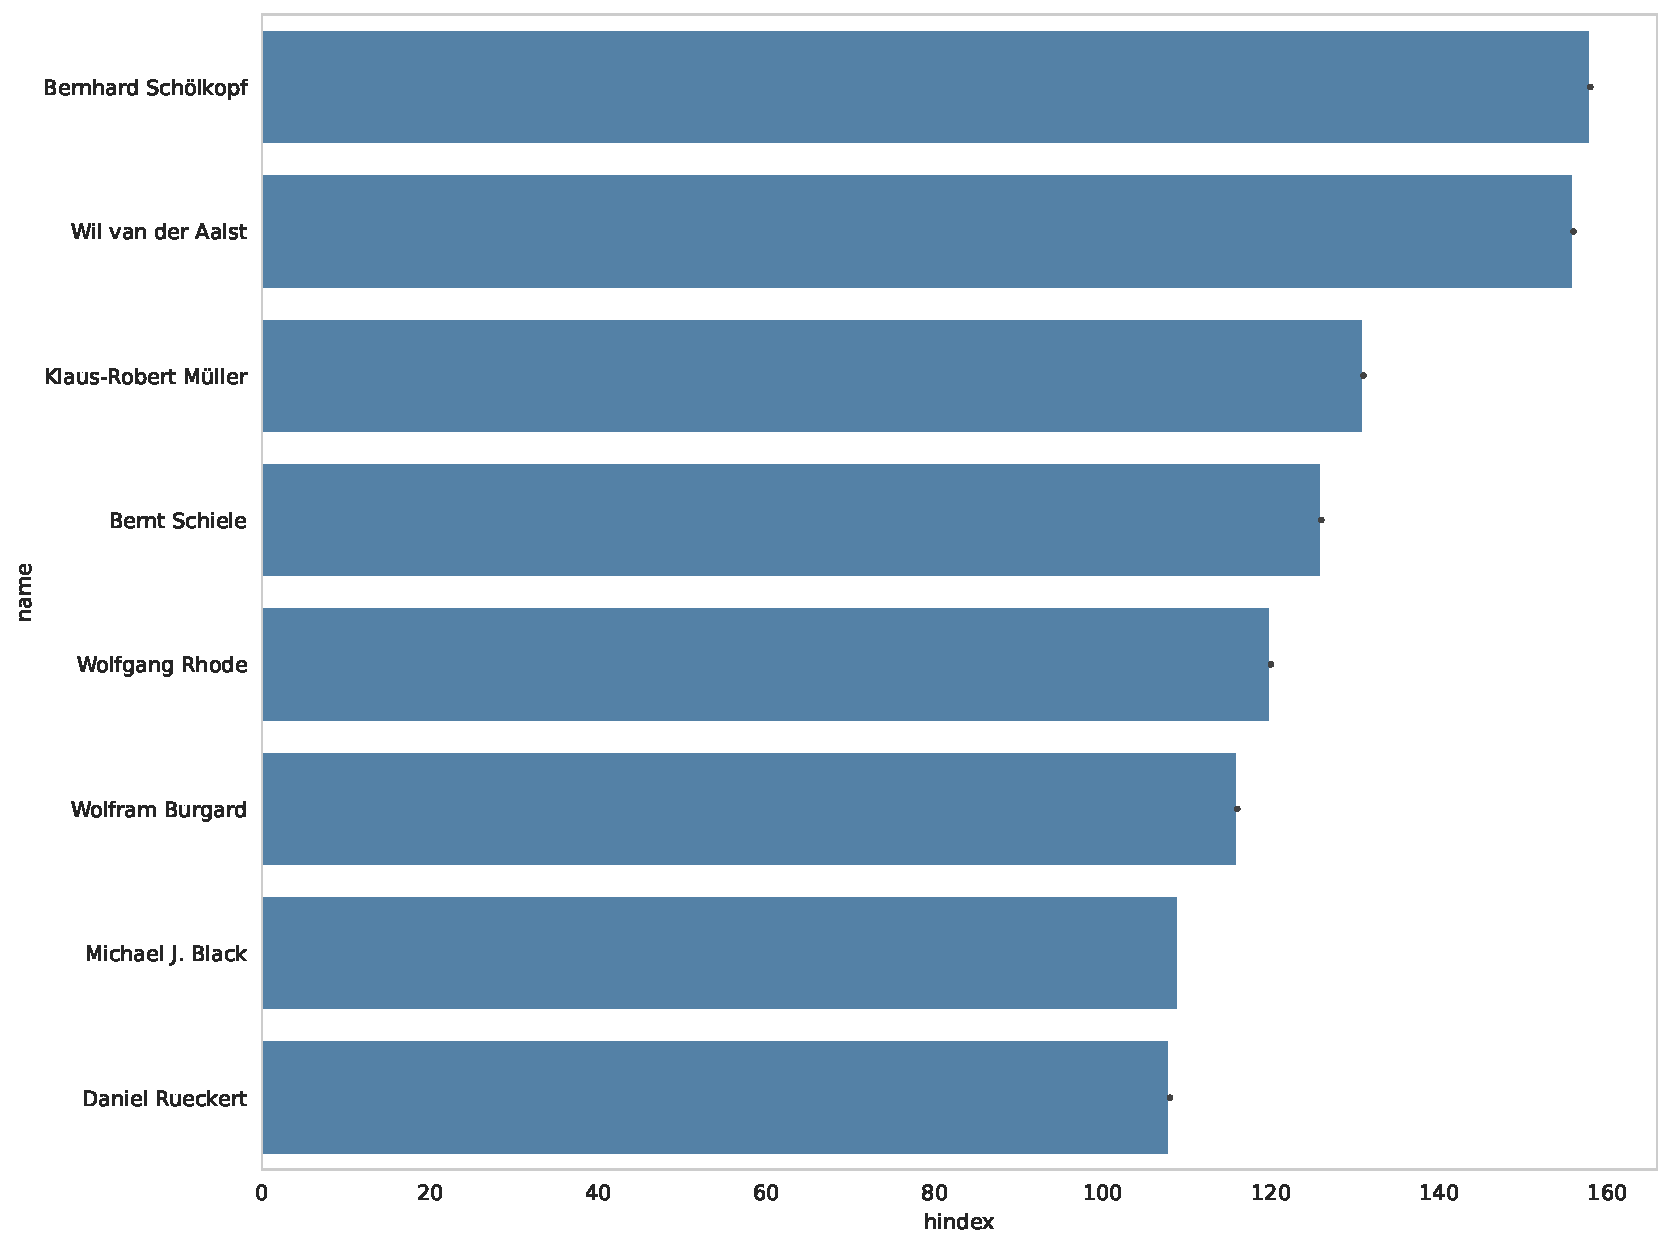
\includegraphics[width=0.8\linewidth]{figures/h-index-top.pdf}
    \caption{Top h-index authors}
    \label{fig:h-index-top}
\end{figure}
\begin{figure}
    \centering
    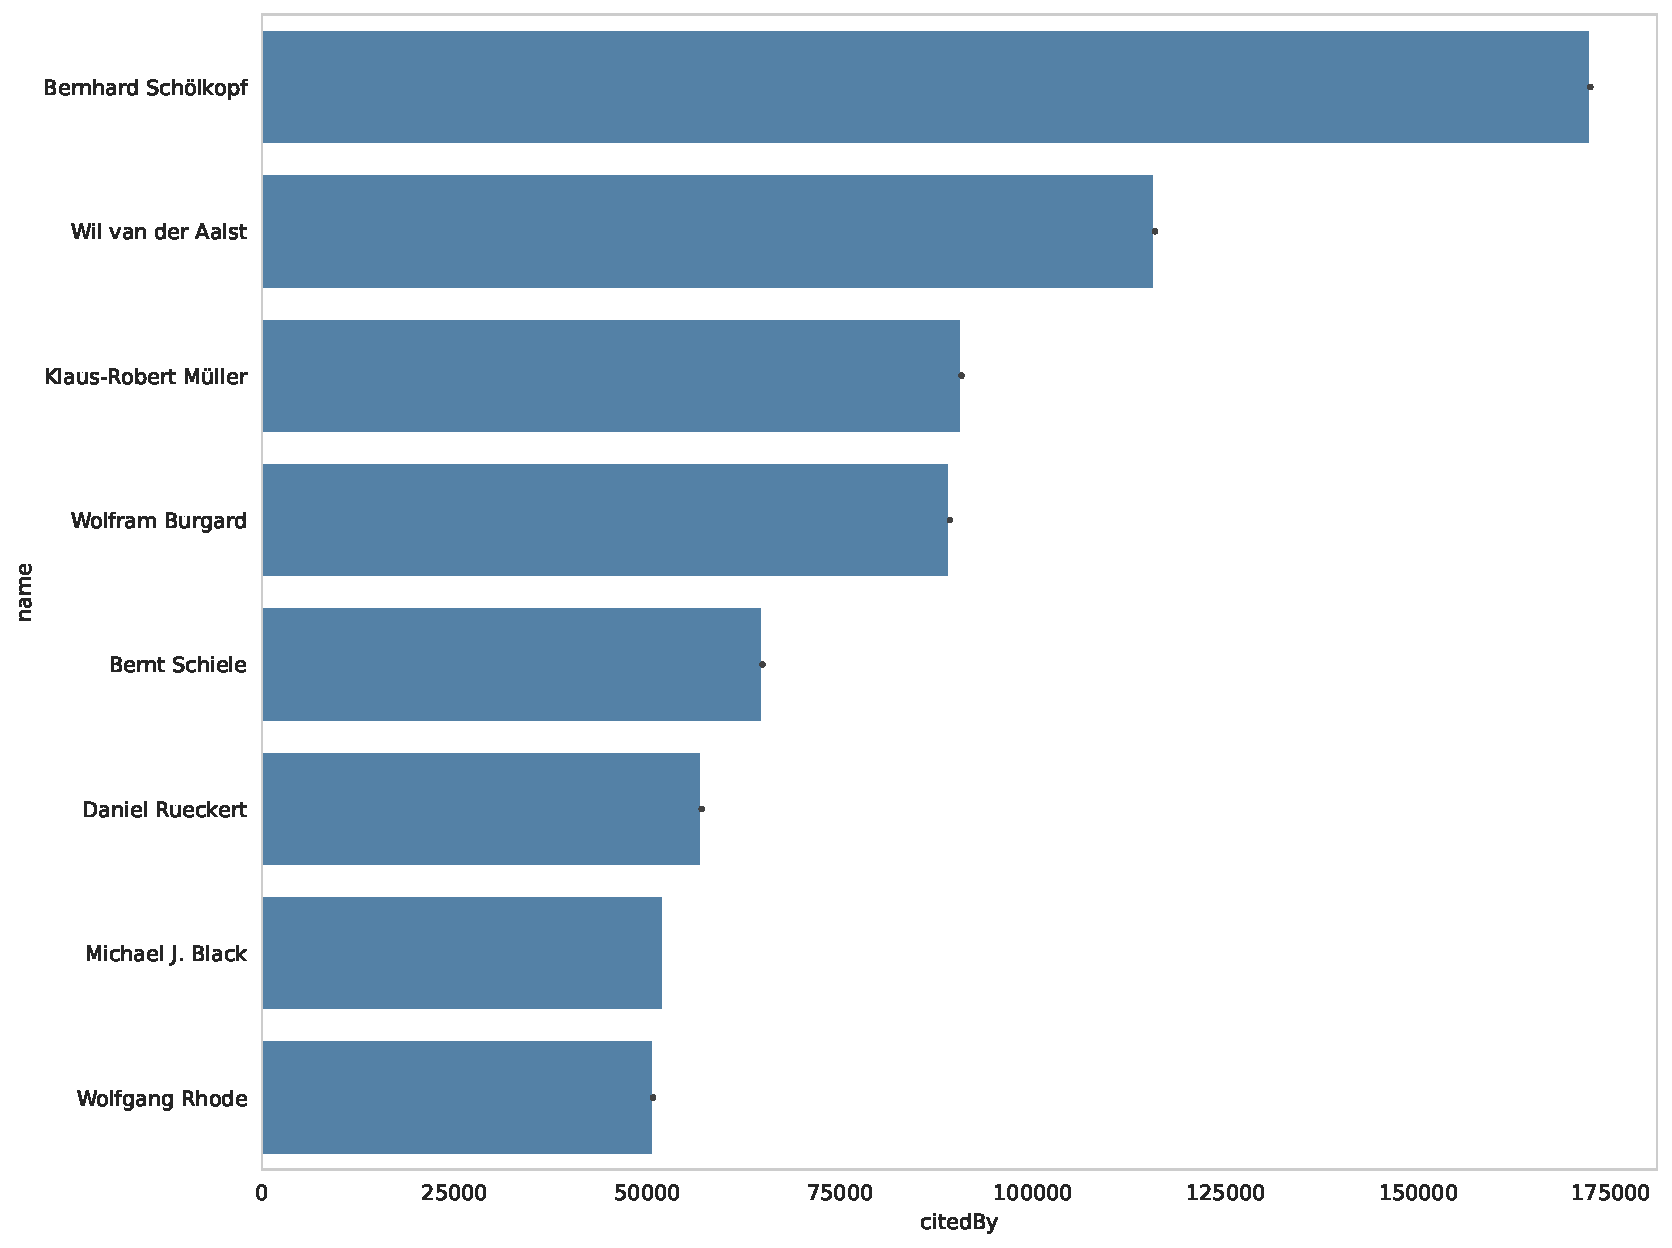
\includegraphics[width=0.8\linewidth]{figures/citeBy-top.pdf}
    \caption{Top CiteBy Authors}
    \label{fig:top-citeBy}
\end{figure}
%\begin{figure}
    \centering
    \includegraphics[width=0.8\linewidth]{figures/mds-scaling.pdf}
    \caption{Multi dimensional scaling of authors based on their keywords}
    \label{fig:mds-scale}
\end{figure}
\end{document}